\section{Exploring the incidents' geographical and temporal distribution}

\subsection*{Question 2.1}
\textit{Do you see a different spatial distribution of incidents over the different years? If so, which are the differences you found?}

Before trying to answer this question, it is interesting to take a closer look to the data.
The data span a temporal period of $9$ years, from $2009$ to $2017$.
The dataset contains $1.441.208$ records, of which $1.027.546$ (about $70\%$) have no information about the time of the incident.
Also, there are only $7$ incidents for year $2009$ and $84$ for year $2010$ (we suspect that many incidents without the time information have happened in these years, but we have no evidence of that).
Our analysis concentrate thus on years $2011$ to $2017$.

Similar to Question 1.2, we use the small multiple design technique.
The visualization is composed of multiple maps: each map shows the incidents in Seattle for a single year.
The maps are sorted in chronological order, i.e. $2011$ is the first on the left, $2017$ the last on the right.
The user is free to change the order to make accurate comparison between pairs of years, if needed.
Since the visualization only shows data for $7$ years, it fits in a single screen.

We use a small size for each point on the map and a medium level of transparency to be able to distinguish areas with different densities.
We use color to overload the encoding of the year:
this allows to combine the visualization with the histogram of incidents' frequency by year, as shown in \cref{fig:2_1_geographical_temporal_distribution} (see dashboard \textit{Incidents geographical and temporal distribution} in Tableau).

\begin{figure}[H]
	\centering
	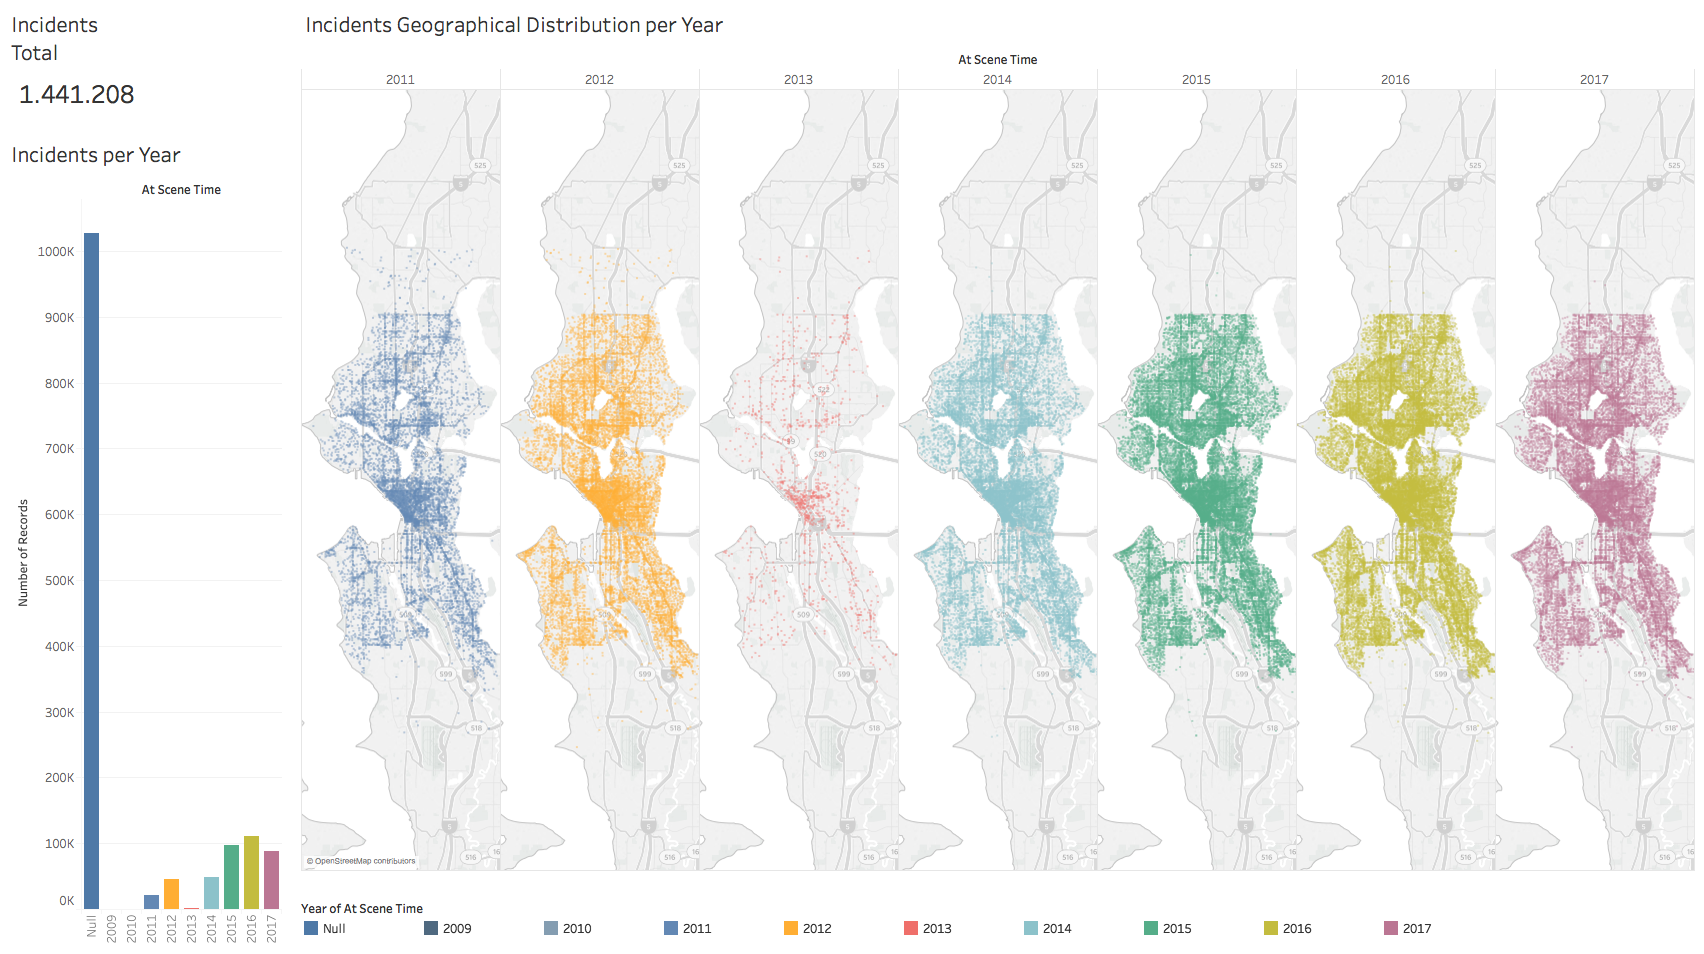
\includegraphics[width=\columnwidth]{figures/2_1_geographical_temporal_distribution}
	\caption{Incidents spatial distribution over different years in Seattle.}
	\label{fig:2_1_geographical_temporal_distribution}
\end{figure}

From the visualization, we can not notice any significant difference in the spatial distribution of incidents over the last $5$ years.
Year $2013$ has significantly less incidents, but this is probably due to the missing temporal information on $70\%$ of the entries.
Anyway, their distribution is similar to the general one: incidents are more concentrated in the city center (see Question 1.1).


\subsection*{Question 2.2}
\textit{Are there zones with a consistent low incidents density over all years? Are there zones with a consistent high density over all years?}

We can use the visualization built for the previous question to answer this one.
Over all years, the city center has a higher concentration of incidents.
Outside the city center, incidents seems to be slightly more concentrated along the main streets.
The distribution in each year is similar to the distribution over all years and is described in greater details in \cref{sec:question1}.
